% NeurIPS 2026: 8th Robot Learning Workshop (WRL)
% Non-archival contributed paper (<=6 pages, NeurIPS format).
% Sister draft: ../icra2027/
%
% Style: official neurips_2026.sty (author kit).
% After acceptance: \usepackage[dblblindworkshop, final]{neurips_2026}

\documentclass{article}

% amsmath before neurips_2026 so it does not clobber NeurIPS \And.
\usepackage{amsmath,amssymb}

% Numeric citations (NeurIPS default natbib is author–year without this).
\PassOptionsToPackage{numbers}{natbib}

% Submission (line numbers; authors omitted for double-blind workshop):
\usepackage[dblblindworkshop]{neurips_2026}
% Camera-ready after accept:
% \usepackage[dblblindworkshop, final]{neurips_2026}

% Do not print the style-file "Anonymous Author(s)" placeholder.
\makeatletter
\renewcommand{\@maketitle}{%
  \vbox{%
    \hsize\textwidth
    \linewidth\hsize
    \vskip 0.1in
    \@toptitlebar
    \centering
    {\LARGE\bf \@title\par}
    \@bottomtitlebar
    \if@anonymous
    \else
      \def\And{%
        \end{tabular}\hfil\linebreak[0]\hfil%
        \begin{tabular}[t]{c}\bf\rule{\z@}{24\p@}\ignorespaces%
      }%
      \def\AND{%
        \end{tabular}\hfil\linebreak[4]\hfil%
        \begin{tabular}[t]{c}\bf\rule{\z@}{24\p@}\ignorespaces%
      }%
      \begin{tabular}[t]{c}\bf\rule{\z@}{24\p@}\@author\end{tabular}%
    \fi
    \vskip 0.3in \@minus 0.1in
  }%
}
\makeatother

\workshoptitle{8th Robot Learning Workshop: Is Physical AI Going Zero-Shot?}

\usepackage[utf8]{inputenc}
\usepackage[T1]{fontenc}
\usepackage{hyperref}
\usepackage{xurl}
\usepackage{booktabs}
\usepackage{amsfonts}
\usepackage{graphicx}
\usepackage{caption}
\usepackage{placeins}
\usepackage{enumitem}
\usepackage{microtype}
\usepackage{xcolor}

\captionsetup{font=small,labelfont=bf,skip=4pt}

% Prefer packing figures with text over nearly empty float pages.
\renewcommand{\topfraction}{0.92}
\renewcommand{\bottomfraction}{0.9}
\renewcommand{\textfraction}{0.07}
\renewcommand{\floatpagefraction}{0.85}
\setcounter{topnumber}{4}
\setcounter{totalnumber}{8}
\setcounter{bottomnumber}{3}

\title{Closing the Frequency Gap:\\
Deploying Vision-Language-Action Models\\
on High-Rate Humanoid Control}

% Omitted on the title page under dblblindworkshop.
% Restored automatically with the [final] option after acceptance.
\author{%
  Osemudiamen Andrew Ihimekpen \And Lijun Qian \\[0.35em]
  {\small Dept.\ of Electrical and Computer Engineering, CREDIT Center}\\
  {\small Prairie View A\&M University, Prairie View, TX, USA}\\
  {\small\texttt{oihimekpen\string@pvamu.edu} \quad \texttt{liqian\string@pvamu.edu}}
}

\begin{document}
\maketitle

\begin{abstract}
Vision-Language-Action (VLA) models make open-vocabulary robot control practical, but their inference rate is often far below the joint-control rates that humanoids need.
We treat this mismatch as a deployment bottleneck rather than a new foundation-model problem.
On a DGX Station (Tesla V100), live \texttt{UnifoLM-VLA-Base} profiling on \texttt{G1\_Clean\_Table} shows a $\sim$57$\times$ gap to 100\,Hz (PyTorch mean \textbf{570.7\,ms} / \textbf{1.752\,Hz}; Nsight NVTX \textbf{593.7\,ms} / \textbf{1.684\,Hz}).
We keep the VLA as a sparse language-conditioned intent generator and insert a fixed Echo State Network (ESN) that turns VLA action commands into smooth 100\,Hz joint commands.
Only a linear readout is trained with ridge regression.
On \texttt{G1\_Dex1\_Wipe\_Table} (200 episodes, train $0$ to $159$ / held-out $160$ to $199$), the CUDA ESN (leak $\alpha{=}0.3$, ridge $\lambda{=}1$) reaches held-out open-loop root-mean-square error (RMSE) \textbf{$2.78\times10^{-3}\!\pm\!3.44\times10^{-3}$\,rad} ($\sim$5.6$\times$ better than linear upsampling) and MuJoCo dataset-oracle RMSE \textbf{$3.00\times10^{-3}\!\pm\!3.56\times10^{-3}$\,rad} (grasp/task success \textbf{100\%}; mean table contact \textbf{74.5\%}).
Live dual-process control clears 100\,Hz on average (ESN mean 6.92\,ms / 145\,Hz).
With matched \texttt{press\_table} priors and motion clamps ($n{=}3$ seeds, 30\,s), live ESN and zero-order hold (ZOH) both succeed, and live joint RMSE is near-tied ($0.521\!\pm\!0.005$ vs.\ $0.532\!\pm\!0.008$\,rad).
The ESN gain that remains clear is offline tracking and jerk, plus the ability to serve the humanoid control loop while the VLA stays sparse.
\end{abstract}

\section{Introduction}
\subsection{Motivation: why VLAs break on humanoids}
Recent VLAs such as RT-2~\cite{RT22023}, OpenVLA~\cite{OpenVLA2025}, Octo~\cite{Octo2024}, and $\pi_0$~\cite{PiZero2024} show that large vision-language backbones can map instructions to robot actions across many tasks and embodiments~\cite{OpenXEmbodiment2024,MaVLASurvey2024}.
Unitree's UnifoLM-VLA~\cite{UnifoLM2026} brings the same idea to a humanoid stack.
That progress is real for semantic control.
It is less clear that the same models are ready for whole-body, contact-rich humanoid loops~\cite{PhysicalAI2025,GR00T2025}.

The Unitree G1 exposes a \textbf{29}-degree-of-freedom (DoF) joint interface that must be served near \textbf{100\,Hz} (10\,ms) for balance-preserving tracking and safe wiping.
Autoregressive and diffusion action heads often spend hundreds of milliseconds on one inference.
If we simply hold each sparse VLA target with ZOH, the robot sees a staircase joint trajectory for tens of control ticks.
That injects high jerk and can ruin contact even when the high-level plan is correct.
We call this the \emph{frequency gap}: the VLA may be right about \emph{what} to do, yet too slow for \emph{how} the humanoid must move.

Two constraints make ``just train a faster VLA'' hard in many labs.
First, the vision-language backbone already saturates common GPUs, so the control layer should stay cheap and preferably avoid backpropagation through time (BPTT).
Second, classical upsamplers (ZOH, linear interpolation, joint proportional-integral-derivative (PID) control toward a held setpoint) ignore proprioception between VLA updates and do not learn demonstration-consistent dynamics.

\subsection{Approach and scope}
We therefore keep UnifoLM as a sparse intent generator ($\sim$1.7\,Hz on our V100) and insert a leaky Echo State Network (ESN) that produces 100\,Hz joint commands.
The reservoir weights stay fixed; only a linear readout is fit by ridge regression on public wipe demonstrations (Sec.~\ref{sec:dataset}).
This is a systems paper about deploying an existing humanoid VLA at control rate, not a claim of zero-shot Physical AI, and not a claim of the first VLA temporal upsample.

\textbf{Contributions.}
To our knowledge, this is the first ridge-trained ESN under a \emph{frozen} humanoid VLA to close a \emph{measured} $\sim$57$\times$ UnifoLM$\rightarrow$G1 rate gap, with held-out tracking and a disclosed live \texttt{press\_table} failure (not the first VLA upsample, and not a new ESN algorithm~\cite{Jaeger2001,Ihimekpen2026}).
\begin{itemize}[leftmargin=1.15em,itemsep=0.2em,topsep=0.3em]
  \item We profile UnifoLM-VLA-Base on \texttt{G1\_Clean\_Table} with two instruments and quantify a $\sim$57 to 59$\times$ gap to 100\,Hz.
  \item We insert a CUDA ESN with input $u(t)=[q_t;\,q^{\star}_{\mathrm{VLA}}]\in\mathbb{R}^{58}$ (current joints $q_t$ and the held VLA target), train only a ridge readout on a declared episode split, and keep a per-task checkpoint library for UnifoLM G1 skills.
  \item We run dual-process MuJoCo timing that bypasses the Python Global Interpreter Lock (GIL) and compare ESN with ZOH, linear interpolation, and joint PID under live UnifoLM.
  \item We evaluate the ESN as a MuJoCo dataset-oracle on all 40 held-out wipe episodes.
  \item We run live UnifoLM wipe trials in simulation with interactive cloth, disclosed geometric priors, matched clamps, and $n{=}3$ seeds, including contact collapse without \texttt{press\_table}.
\end{itemize}

\section{Related work}
\textbf{Generalist robot policies.}
Large-scale robot datasets and RT-X models~\cite{OpenXEmbodiment2024} catalyzed open generalist policies such as Octo~\cite{Octo2024} and OpenVLA~\cite{OpenVLA2025}.
Flow-matching VLAs such as $\pi_0$~\cite{PiZero2024} push action generation further, and recent surveys map the remaining gaps for embodied AI~\cite{MaVLASurvey2024,PhysicalAI2025}.
Humanoid-oriented stacks such as UnifoLM~\cite{UnifoLM2026} and GR00T~\cite{GR00T2025} make the control-rate question concrete: semantic competence is not the same as a 100\,Hz whole-body loop.

\textbf{Action generation and temporal structure.}
Diffusion Policy~\cite{DiffusionPolicy2023} and action chunking~\cite{ACT2023} improve smoothness by predicting action sequences rather than single steps.
Memory-augmented VLAs explore longer horizon structure~\cite{Notes2Self2026}.
Faster or smaller VLAs such as TinyVLA~\cite{TinyVLA2024} attack latency inside the policy.
We take a complementary route: leave the foundation VLA sparse, and add a light dynamical bridge underneath it.
That is not the first way to upsample or smooth VLA actions; it is a training-light alternative that leaves the backbone frozen.

\textbf{Reservoir computing for fast control.}
Echo State Networks provide trainable-light temporal filtering with fixed recurrent weights~\cite{Jaeger2001,Caoetal2023}.
Ihimekpen et al.\ showed that a fixed reservoir with a ridge-trained readout can identify and control spring-mass systems with switched dynamics~\cite{Ihimekpen2026}.
We reuse that training-light property (not a new ESN algorithm) to close the measured UnifoLM-to-G1 rate gap, without backpropagating through the reservoir.

\section{Method}
\subsection{System architecture}
Figure~\ref{fig:architecture} shows the hybrid stack.
Frozen UnifoLM emits sparse 23-D end-effector (EE) intents.
A Jacobian inverse-kinematics (IK) bridge lifts them to 29-D joint targets and holds $q^{\star}$ for 50 ticks.
A fixed ESN reservoir with a ridge-trained readout then produces 100\,Hz MuJoCo PD commands conditioned on current joints.

\begin{figure}[t]
\centering

\includegraphics[width=\linewidth]{figures/fig1_architecture.png}
\caption{Two-rate VLA$+$ESN stack on simulated G1 (29\,DoF). Frozen UnifoLM-VLA-Base ($\sim$1.75\,Hz, V100) emits 23-D EE chunks; Jacobian IK holds $q^{\star}$ for 50 ticks. Only $W_{\mathrm{out}}$ is trained. Process~B closes the $\sim$57$\times$ gap with 100\,Hz MuJoCo PD.}
\label{fig:architecture}
\end{figure}

\begin{itemize}[leftmargin=1.15em,itemsep=0.2em,topsep=0.3em]
  \item \textbf{Perception / VLA:} Frozen \texttt{UnifoLM-VLA-Base} consumes RGB, language, and 23-D EE proprioception, and emits 23-D EE action chunks.
  A Jacobian IK bridge maps EE \emph{xyz} to 29-D $q^{\star}$ (legs held) and latches the target for 50 ticks.
  \item \textbf{ESN bridge:} Leaky reservoir
  \[
  x(t)=(1-\alpha)x(t-1)+\alpha\,\tanh\!\big(W_{\mathrm{res}}x(t-1)+W_{\mathrm{in}}u(t)\big),
  \]
  with reservoir state $x(t)$, leak rate $\alpha$, sparse reservoir weights $W_{\mathrm{res}}$ (size $N{=}1000$, spectral radius $\rho{=}0.95$, sparsity $0.9$), and input weights $W_{\mathrm{in}}$.
  The readout $y(t)=W_{\mathrm{out}}[x(t);u(t)]$ is fit by ridge regression (penalty $\lambda$) on 100\,Hz joints with VLA tokens held for 50 ticks ($u\in\mathbb{R}^{58}$, $y\in\mathbb{R}^{29}$).
  We sweep $\alpha\in\{0.05,0.1,0.3\}$ and $\lambda\in\{10^{-4},10^{-2},1\}$ and select by an RMSE$\times$jerk score.
\end{itemize}

\subsection{Baselines}
We compare four bridges under the same sparse VLA intents:
(1)~pure VLA ZOH,
(2)~VLA $+$ linear interpolation,
(3)~VLA $+$ joint PID toward the held target,
(4)~VLA $+$ ESN (ours).

\section{Experiments}
\subsection{Dataset, setup, and metrics}
\label{sec:dataset}
ESN training, offline upsample baselines, and MuJoCo wipe-oracle evaluations use
\texttt{G1\_Dex1\_Wipe\_Table} from \texttt{unitreerobotics} (Hugging Face \texttt{train} split):
\textbf{200} episodes ($75{,}909$ frames; $\sim$0.70\,h), train episodes $0$ to $159$ / held-out $160$ to $199$.
We keep detailed wipe claims inside this corpus, while the training stack also supports a per-task ESN library over other UnifoLM G1 skills.
Figure~\ref{fig:dataset} shows the episode-length distribution and the episode-level 80/20 split.
Hardware is a Unitree G1 (29\,DoF) simulated stack on an NVIDIA DGX Station (Tesla V100-DGXS-32GB).
Profiling uses live UnifoLM-VLA-Base on G1 Clean-Table in half precision (FP16).
We report task success (grasp / wipe contact), joint RMSE, trajectory jerk, and control rate.

Three evaluation settings are kept separate.
Open-loop RMSE compares ESN (or baseline) joint commands to held-out demonstration joints.
The MuJoCo dataset-oracle replays those tokens in simulation.
Live wipe runs UnifoLM and the bridge in MuJoCo with interactive cloth.
None of these is hardware closed-loop control.
Reported $\pm$ values are standard deviations over held-out episodes or live seeds.

\subsection{Results}
Table~\ref{tab:measured} summarizes the measurements.
Table~\ref{tab:offline} isolates held-out tracking and jerk, which is where ESN separates from classical upsamplers.
Table~\ref{tab:multitask} checks that the same bridge stays in a low open-loop RMSE regime on two additional UnifoLM G1 skills.
Figures~\ref{fig:latency} to~\ref{fig:contact} show the latency gap, dataset split, offline baselines, live timing, and the contact ladder.

\begin{figure}[t]
\centering
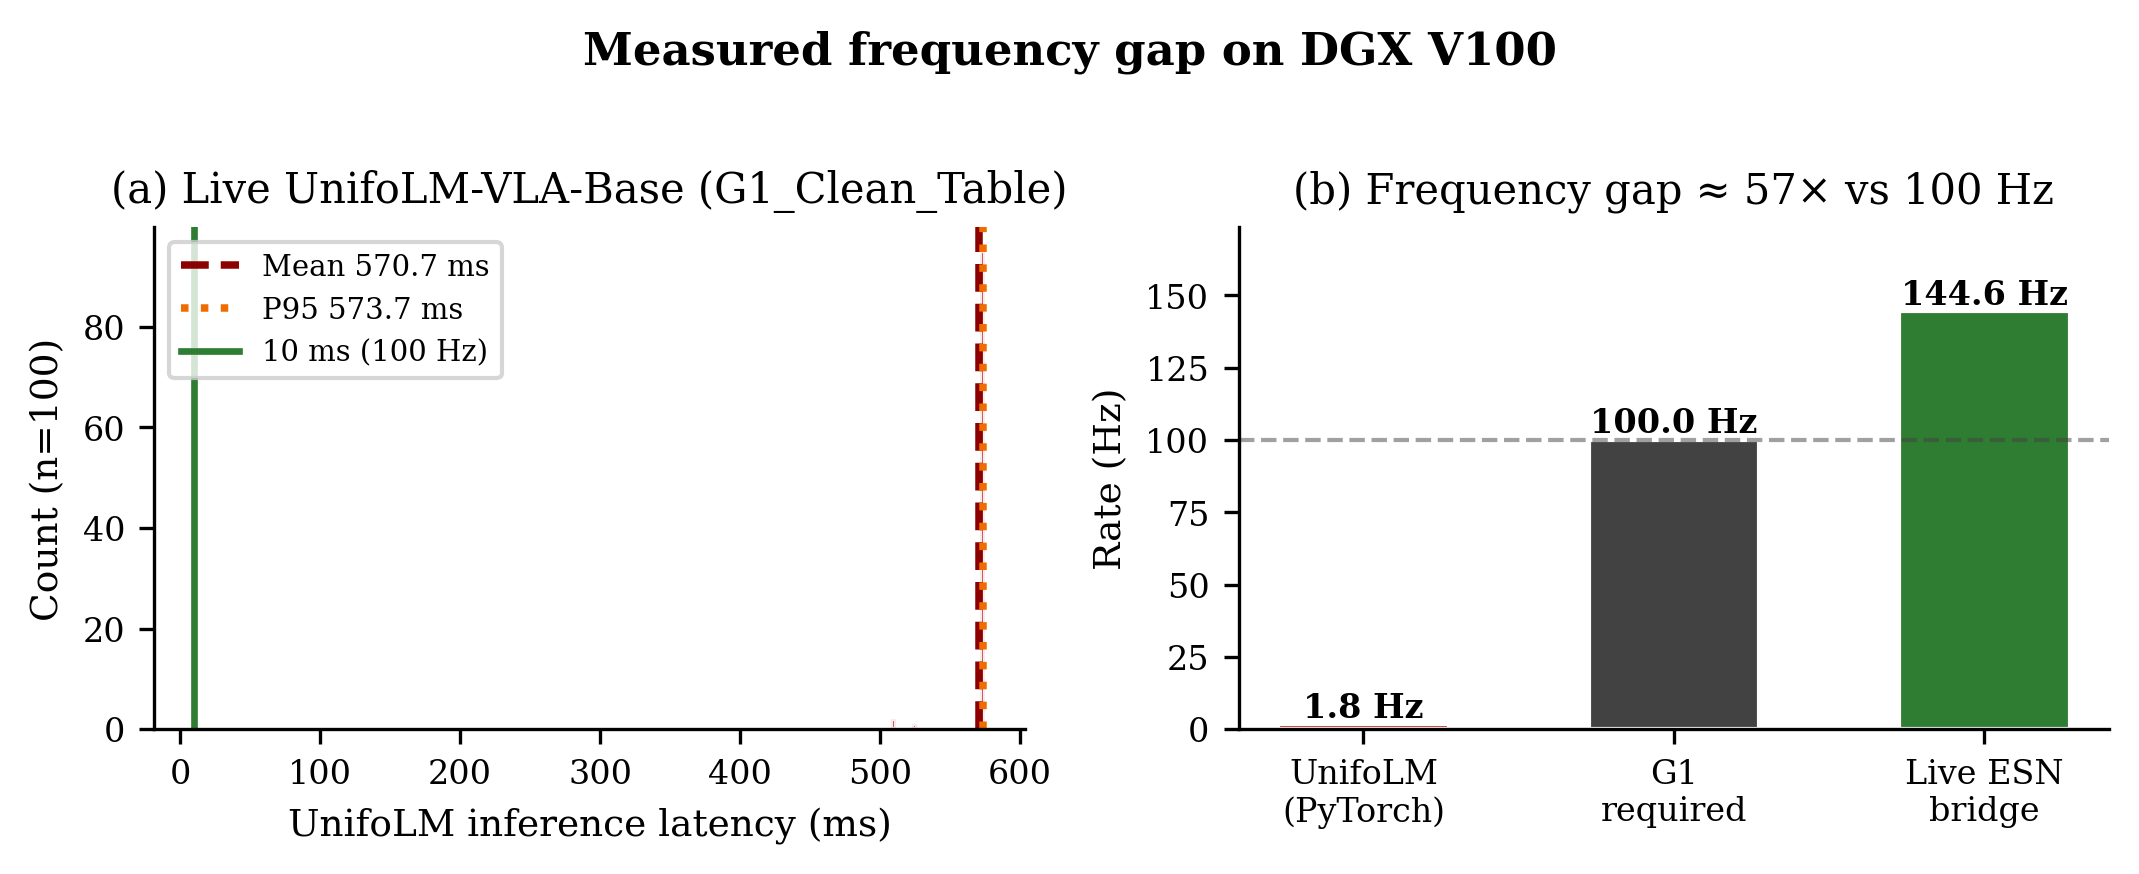
\includegraphics[width=\linewidth]{figures/fig2_latency_gap.png}
\caption{Measured UnifoLM frequency gap on DGX V100 (PyTorch $n{=}100$ on \texttt{G1\_Clean\_Table}): mean 570.7\,ms / 1.752\,Hz vs.\ the 100\,Hz G1 budget; live ESN dual-process clears 100\,Hz mean.}
\label{fig:latency}
\end{figure}

\begin{figure}[t]
\centering
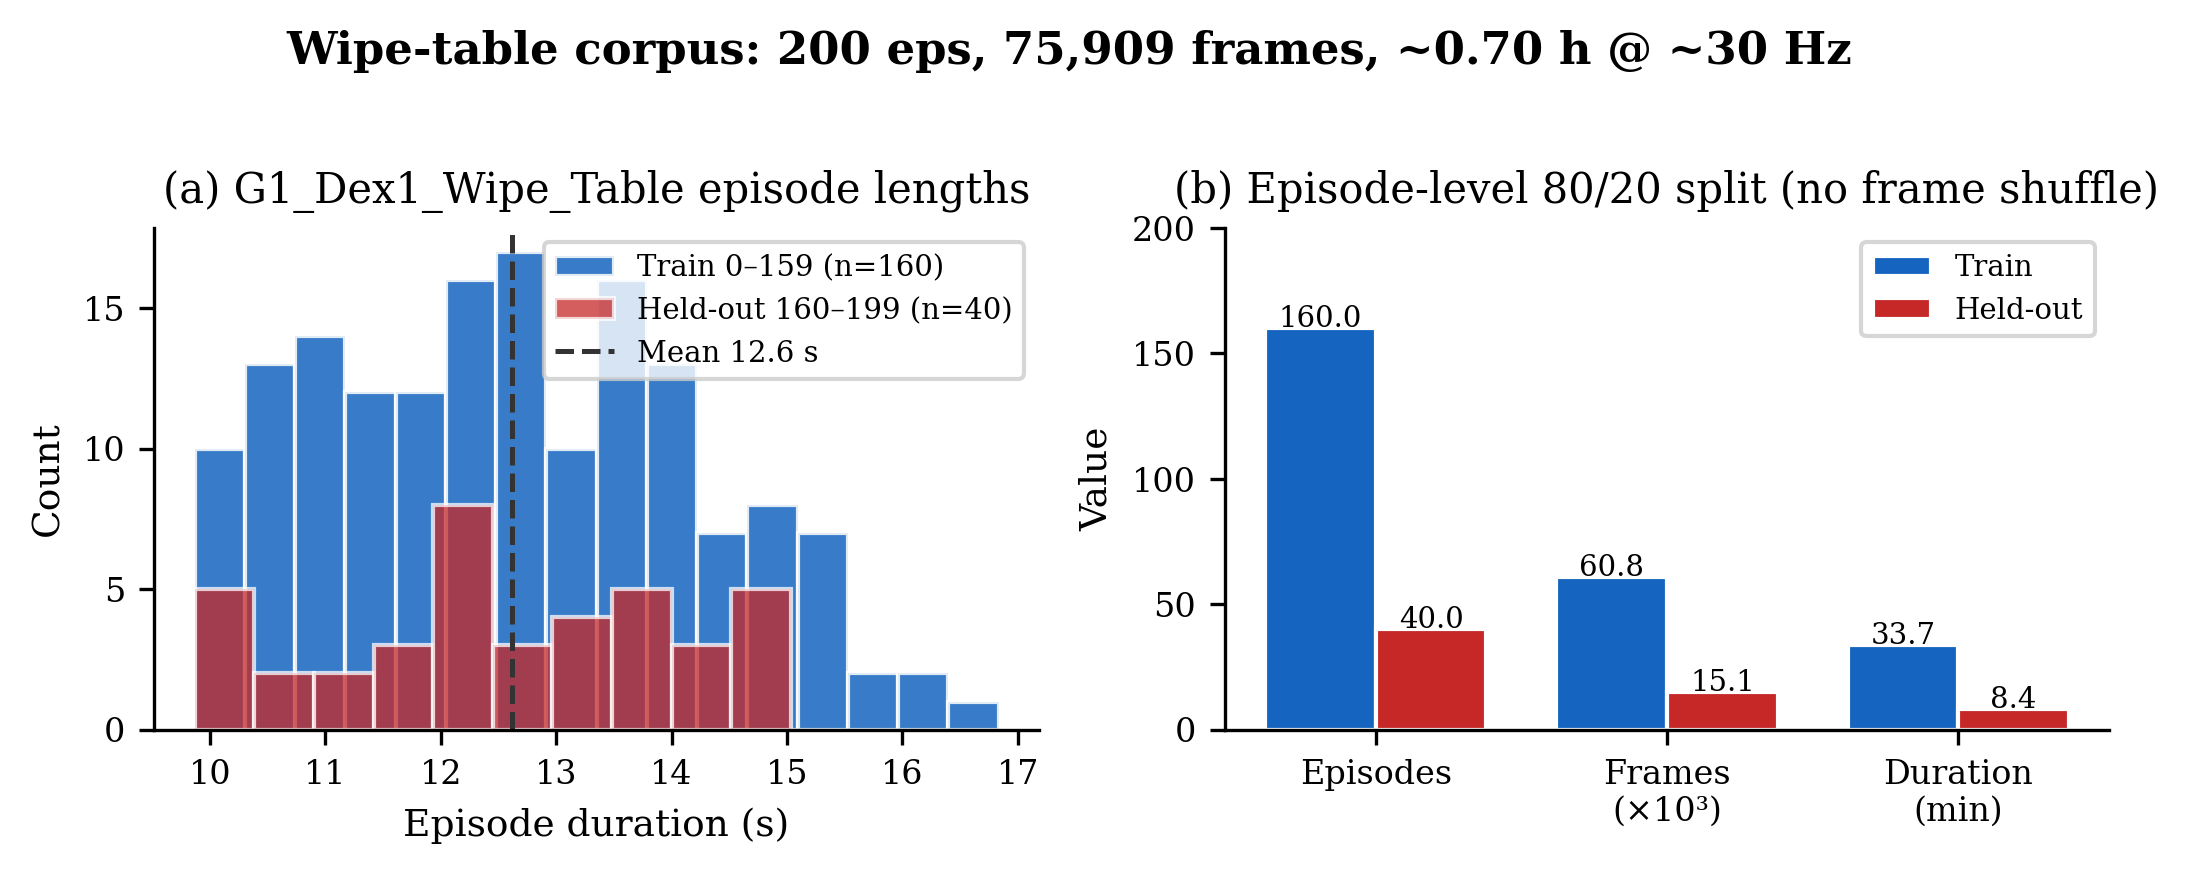
\includegraphics[width=\linewidth]{figures/fig3_dataset_distribution.png}
\caption{Wipe-table corpus used for all ESN / baseline / oracle claims: episode durations and the episode-level 80/20 train ($0$ to $159$) / held-out ($160$ to $199$) split on \texttt{G1\_Dex1\_Wipe\_Table}.}
\label{fig:dataset}
\end{figure}

\begin{table}[t]
\centering
\caption{Summary of measured results.}
\label{tab:measured}
\small
\setlength{\tabcolsep}{4pt}
\begin{tabular}{@{}ll@{}}
\toprule
\textbf{Measurement} & \textbf{Result} \\
\midrule
VLA latency (PyTorch, $n{=}100$) & 570.7\,ms / 1.75\,Hz ($57\times$ below 100\,Hz) \\
VLA latency (Nsight) & 593.7\,ms / 1.68\,Hz \\
ESN held-out RMSE & $2.78\times10^{-3}\!\pm\!3.44\times10^{-3}$\,rad \\
ESN vs.\ linear RMSE & $\sim$5.6$\times$ lower \\
Live ESN step time & 6.92\,ms / 145\,Hz \\
MuJoCo oracle ($n{=}40$) & 100\% grasp; 74.5\% contact \\
Live wipe RMSE (ESN vs.\ ZOH) & $0.521\!\pm\!0.005$ vs.\ $0.532\!\pm\!0.008$\,rad (tied) \\
\bottomrule
\end{tabular}
\end{table}

\begin{table}[t]
\centering
\caption{Held-out joint tracking on wipe episodes 160 to 199.}}
\label{tab:offline}
\small
\setlength{\tabcolsep}{6pt}
\begin{tabular}{@{}lcc@{}}
\toprule
\textbf{Method} & \textbf{RMSE (rad)} & \textbf{Jerk vs.\ linear} \\
\midrule
ZOH & $5.39\times10^{-2}\!\pm\!9.44\times10^{-3}$ & $50\times$ \\
Linear & $1.55\times10^{-2}\!\pm\!3.93\times10^{-3}$ & $1$ \\
PID & $7.14\times10^{-2}\!\pm\!1.19\times10^{-2}$ & $1.43\times$ \\
\textbf{ESN (ours)} & $\mathbf{2.78\times10^{-3}\!\pm\!3.44\times10^{-3}}$ & $1.44\times$ \\
\bottomrule
\end{tabular}
\end{table}

\begin{table}[t]
\centering
\caption{Held-out ESN joint RMSE on three tasks (open-loop tracking).}
\label{tab:multitask}
\small
\setlength{\tabcolsep}{6pt}
\begin{tabular}{@{}llc@{}}
\toprule
\textbf{Task} & \textbf{Episodes} & \textbf{RMSE (rad)} \\
\midrule
Wipe table & 40 & $2.78\times10^{-3}\!\pm\!3.44\times10^{-3}$ \\
Clean table & 40 & $3.68\times10^{-3}\!\pm\!6.72\times10^{-3}$ \\
Stack block & 40 & $4.25\times10^{-3}\!\pm\!2.84\times10^{-3}$ \\
\bottomrule
\end{tabular}
\end{table}

\begin{figure}[t]
\centering
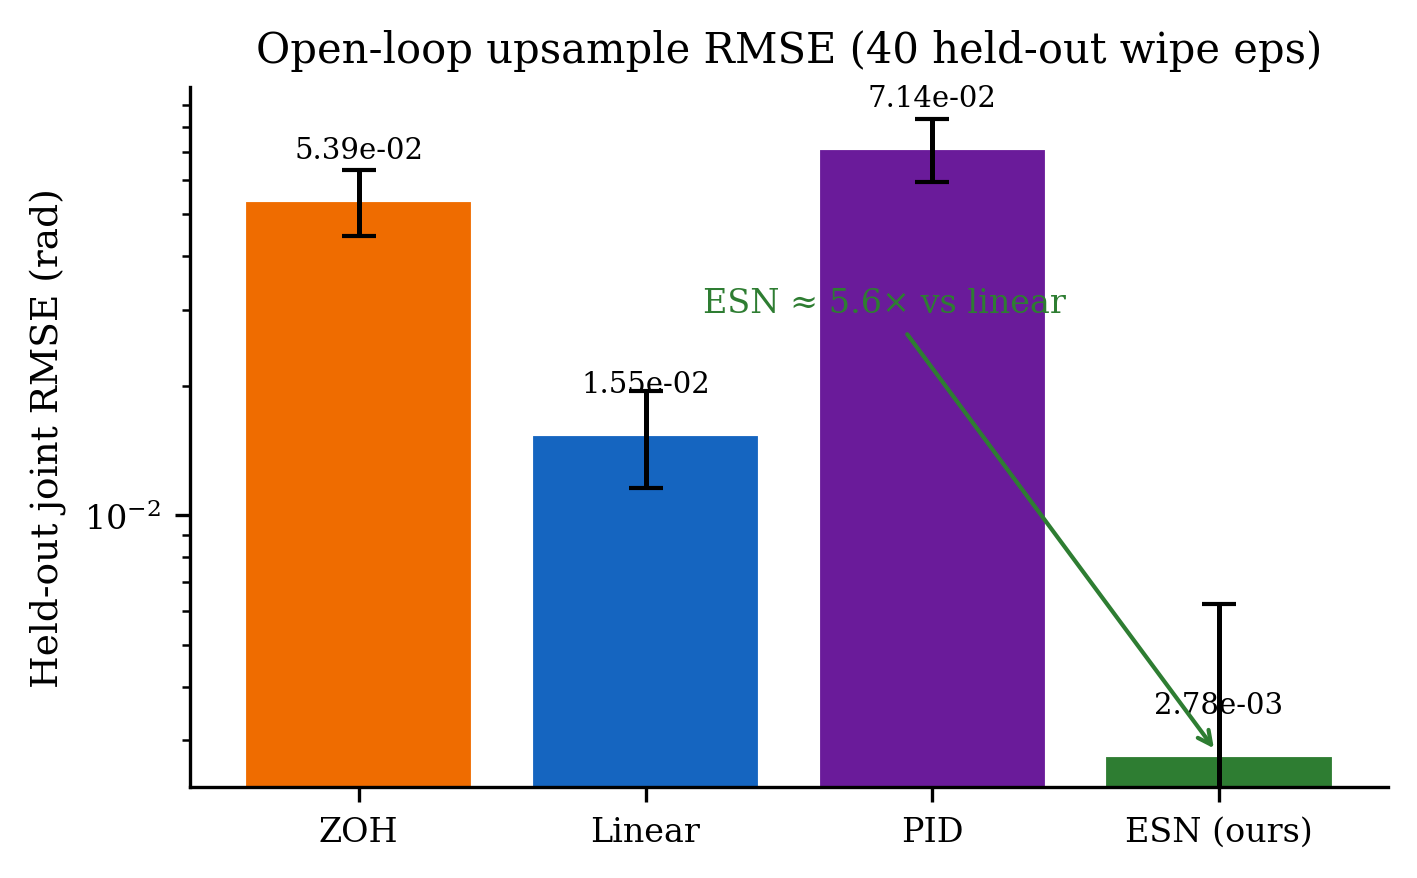
\includegraphics[width=0.78\linewidth]{figures/fig4_offline_baselines.png}
\caption{Open-loop held-out RMSE on wipe episodes 160 to 199 (log scale): ESN is $\sim$5.6$\times$ lower than linear upsampling.}
\label{fig:baselines}
\end{figure}

\begin{figure}[t]
\centering
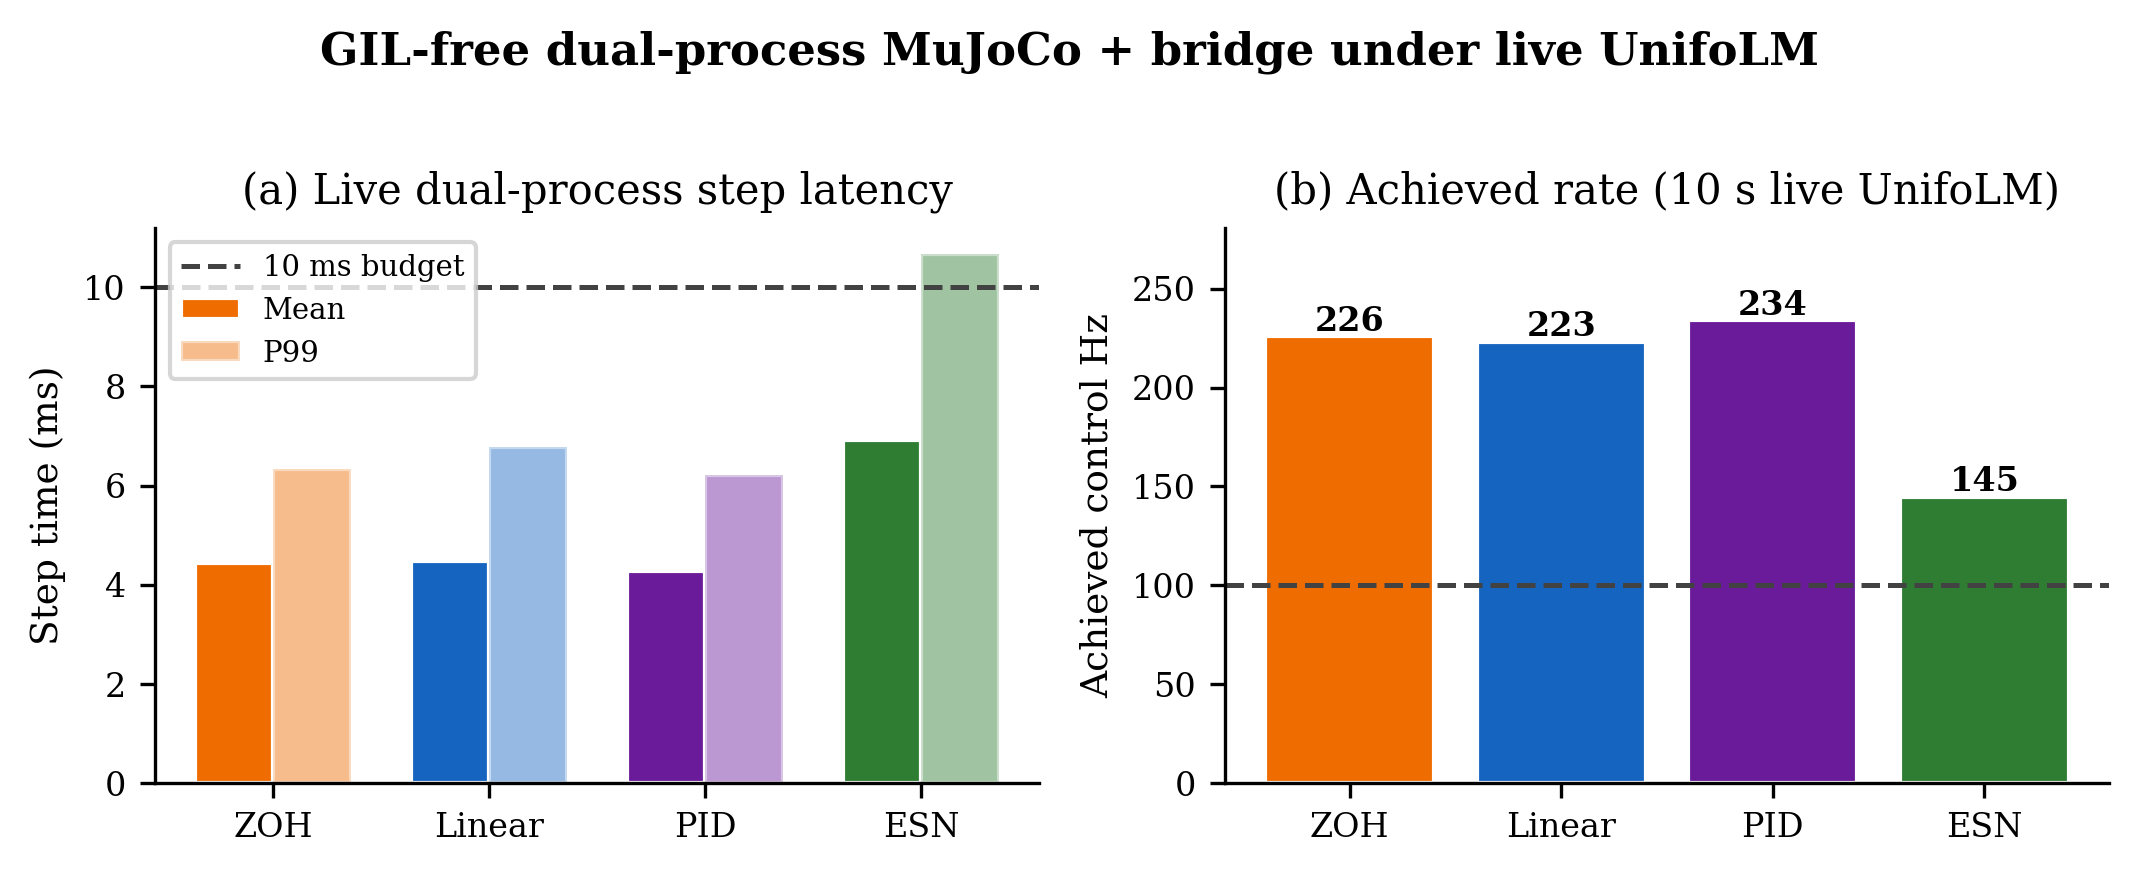
\includegraphics[width=\linewidth]{figures/fig7_control_rates.png}
\caption{Live dual-process MuJoCo$+$bridge under UnifoLM (10\,s): mean/P99 step latency and achieved control Hz for ZOH, linear, PID, and ESN.}
\label{fig:rates}
\end{figure}

\FloatBarrier
\section{Discussion and limitations}
\begin{center}
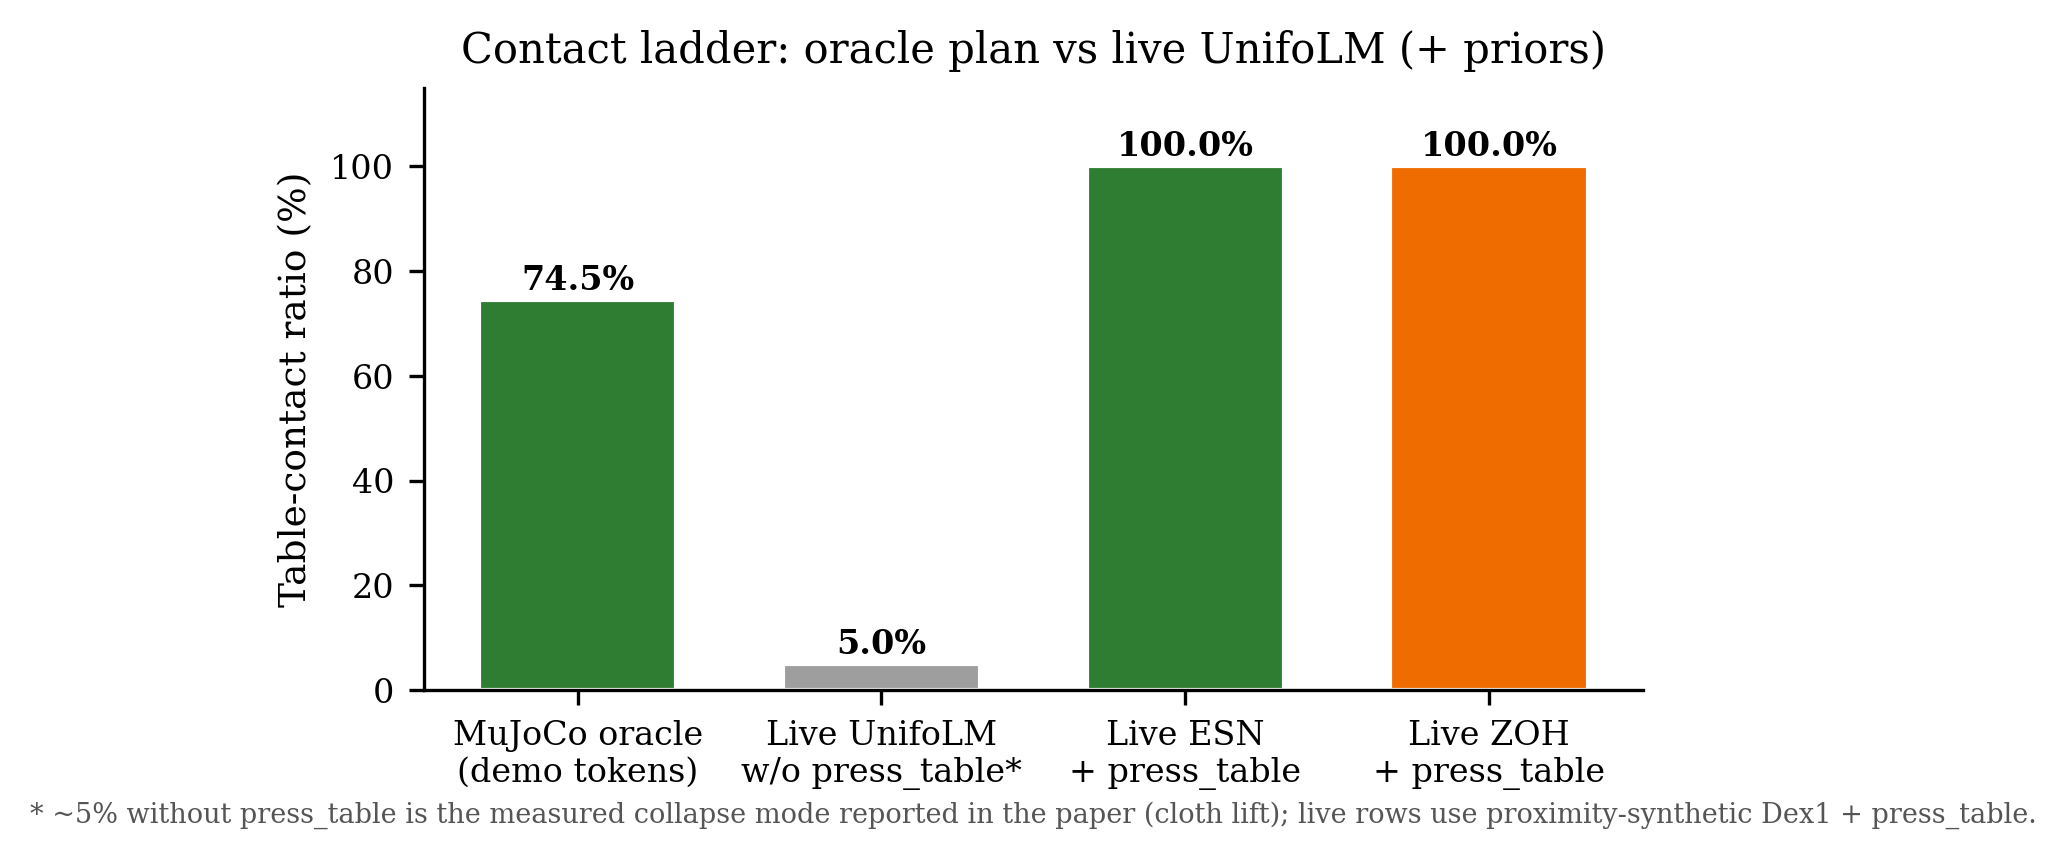
\includegraphics[width=0.78\linewidth]{figures/fig6_contact_ladder.png}
\captionof{figure}{Contact ladder: oracle demo tokens (74.5\%) vs.\ live UnifoLM without \texttt{press\_table} ($\sim$5\% collapse) vs.\ live ESN/ZOH with a disclosed geometric press prior (100\%).}
\label{fig:contact}
\end{center}
\paragraph{Frequency gap.}
Two independent profilers agree on a $\sim$57 to 59$\times$ gap to 100\,Hz.
Both point to large general matrix multiplies (GEMMs) as the dominant cost; Nsight also highlights host-to-device pressure.
That is why we keep the VLA sparse and put a cheap bridge on the joint loop.

\paragraph{Data scope.}
Training and the primary live wipe trials use one task and about 0.7\,h of Dex1 demonstrations with an episode-level 80/20 split.
Open-loop held-out joint RMSE also stays in the $10^{-3}$\,rad regime on clean-table and stack-block (Table~\ref{tab:multitask}), which suggests the bridge is not wipe-only.
That comparison is open-loop tracking of demonstration joints, not live multi-task control, and it does \emph{not} show zero-shot humanoid competence.

\paragraph{What ESN wins, and what stays tied.}
Offline, ESN is $\sim$5.6$\times$ better than linear upsampling and much less jerky than ZOH (Table~\ref{tab:offline}).
That remains the clearest empirical reason to prefer the reservoir.
Live, the dual-process ESN clears 100\,Hz on average (145\,Hz mean), with GPU-contention tails above 10\,ms when UnifoLM shares the device.
On interactive cloth, removing the table-plane press prior collapses contact to about 5\%.
With matched \texttt{press\_table} priors and motion clamps over $n{=}3$ seeds (init eps 160/170/180, 30\,s), both ESN and ZOH reach 100\% contact and task success, and live joint RMSE is near-tied ($0.521\!\pm\!0.005$ vs.\ $0.532\!\pm\!0.008$\,rad).
So we do not claim a live joint-RMSE win under identical clamps.
We do claim a practical deployment pattern: use the VLA for sparse intent, use a light dynamical bridge for rate, and report the geometric priors that still decide contact success.

\paragraph{Onboard sensing field of view.}
Live G1 head-camera bring-up (RGB$+$depth over ZMQ at $\sim$10\,Hz) shows a strongly downward ego view: floor and near-field workspace dominate, with little forward horizon.
That is a deployment challenge for any vision-conditioned outer loop and is independent of the ESN bridge.
Hardware transfer therefore needs camera pitch / mount checks, and possibly wrist or multi-view inputs, before a vision-conditioned wipe can be claimed on the robot.

\section{Conclusion}
We studied the frequency gap between UnifoLM-VLA-Base inference and G1 100\,Hz control as a Physical AI deployment problem.
To our knowledge, this is the first ridge-trained ESN under a frozen humanoid VLA used to close that \emph{measured} $\sim$57$\times$ UnifoLM$\rightarrow$G1 gap, with held-out tracking and a disclosed live \texttt{press\_table} failure.
We do not claim the first VLA upsample, a new ESN method, or a live RMSE win: under matched priors and clamps in simulation, ESN and ZOH succeed together.
The remaining ESN evidence is offline tracking and jerk, plus a joint loop that stays at 100\,Hz while the VLA stays sparse.
Evaluating the stack on a physical G1 is the natural next step.

\begin{ack}
Supported in part by ARO Cooperative Agreement W911NF-24-2-0133.
\end{ack}

\bibliographystyle{unsrtnat}
{\small
\bibliography{references}
}

\end{document}
